\documentclass[12pt,a4paper]{article}
\usepackage[utf8]{inputenc}
\usepackage{graphicx}
% Document config
\usepackage[letterpaper, margin=1in]{geometry}
\usepackage[spanish]{babel}
\usepackage[utf8]{inputenc}
\usepackage{tikz}
\usepackage{hyperref}
\usepackage{minted,xcolor}
\usemintedstyle{tango}
\usepackage{color}
\usepackage{xcolor}
\usepackage{float}
\usepackage{tcolorbox}
\usepackage[nottoc]{tocbibind}
\usepackage{graphicx}
\usepackage{listings}
\usepackage{lineno}
\usepackage{fancyvrb}
\usepackage{minted}
\usepackage[utf8]{inputenc}
\usepackage{pdfpages} %para importar paginas de un pdf
\usepackage{multirow}
\addto\captionsspanish{\renewcommand{\listtablename}{Índice de tablas}}		% Cambiar nombre a lista de tablas   
\addto\captionsspanish{\renewcommand{\tablename}{Tabla}}					% Cambiar nombre a tablas
\usepackage{float}		% Para ubicar las tablas y figuras justo después del texto
\usepackage{pdfpages}
\usepackage{enumerate}%listas y viñetas

\usepackage{parskip}
\usepackage{circuitikz}
\usepackage{siunitx}
\usepackage{hyperref}
%%%%%%%%%%%%%%%%%%%%%%%%%%%%%%%%%%%%%%%%%%%%%%%%%%%%%%%%%%%%%%%%%%%%
\title{
{

    \begin{tikzpicture}[overlay, remember picture]
        \node[anchor=north west, %anchor is upper left corner of the graphic
            xshift=3cm, %shifting around
            yshift=-4cm] 
            at (current page.north west) %left upper corner of the page
        {
\includegraphics[height=1.3cm]{logoEIE.png}}; 
    \end{tikzpicture}
    \begin{tikzpicture}[overlay, remember picture]
        \node[anchor=north east, %anchor is upper left corner of the graphic
            xshift=-2.5cm, %shifting around
            yshift=-4cm] 
            at (current page.north east) %left upper corner of the page
        {
\includegraphics[height=1.3cm]{logoUCR.png}}; 
    \end{tikzpicture}
    \Large 
        \textbf{Universidad de Costa Rica}\\
        Facultad de Ingeniería\\
        Escuela de Ingeniería Eléctrica\\~\\ \vspace{2cm}
        \texttt{IE-0117}\\Programación Bajo Plataformas Abiertas \\
    }
    ~\\~\\
    {\LARGE \textbf{Laboratorio \#7 \vspace{0cm}}}}
    
\author{Fernando Jiménez Ureña B74020\\ Cristopher Bolaños B31044}
\\
\date{II ciclo\\Noviembre 2021 } 

%%%%%%%%%%%%%%%%%%%%%%%%%%%%%%%%%%%%%%%%%%%%%%
\usepackage{fancyhdr}
\pagestyle{fancy}
\setlength{\headheight}{14.49998pt}

\lhead{IE0117-Programación Bajo Plataformas Abiertas}
\chead{}
\rhead{Laboratorio \#7}
\lfoot{Universidad de Costa Rica}
\cfoot{\thepage}
\rfoot{Escuela de Ingeniería Eléctrica}
%%%%%%%%%%%%%%%%%%%%%%%


%%%%%%%%%%%%%%%%%%%%%%%%%%%%%%%%%%%%%

\begin{document}
%%%%%%%%%%%%%%%%%%%%%%%%%%%%%%%%%%%%%%%%%%%%%%%%%%%%%%%%%%%
\maketitle
\thispagestyle{empty}%%no formato a la portada
\renewcommand{\thepage}{\roman{page}}
\newpage
%%%%%%%%%%%%%%%%%%%%%%%%%%%%%%%%%%%%%%%%5
\renewcommand{\thepage}{\arabic{page}} 
\setcounter{page}{1}

\newpage


%%%%%%%%%%%%%%%%%%%%%%%%%%%%%%%
\newpage
\section{Resumen}

En el presente Laboratorio, se busca poner en práctica todos los conceptos aprendidos en el curso sobre el bloque del lenguaje de programación C. Durante el desarrollo del laboratorio se pondrá en práctica temas como punteros, memoria dinámica, funciones, estructuras, listas enlazadas y entre otras. 

\section{Nota Teórica}

A pesar de que se utilizarán todos los conceptos aprendidos en el bloque de C, sobresalen dos temas esenciales para el desarrollo del laboratorio. Estos temas son la estructura de datos y listas enlazadas. Por su complejidad, se investigará más a fondo los conceptos de cada uno ya que como fue mencionado anteriormente, serán esenciales para el desarrollo de este laboratorio ya que se acudirá a sus algoritmos de manera seguida. Además es importante mencionar que la parte teórica del resto de conceptos ya fue explicada y desarrollada en los laboratorios anteriores.

En el proceso de aprendizaje del lenguaje de programación C, se ha podido apreciar la existencia de diversos tipos de datos con los que se puede manipular, entre ellos: enteros, flotantes y caracteres. Se ha notado que para manipular de mejor manera dichos datos, existen los arreglos comúnmente como \textit{arrays} o \textit{vectores}. No obstante, estos arreglos poseen una gran limitante debido a que no se pueden mezclar estos tipos de datos entre sí.

A medida que se desean realizar procesos más complejos, se desea que a la hora de manipular datos, éstos puedan mezclarse entre sí. Un ejemplo de esto, es cuando se desea conocer y manejar todos los números de identificación, nombres y, direcciones de todos los usuarios de un sistema. Este proceso, puede simplificarse con el uso de estructuras de datos ya que es muy simple definir una serie de posiciones en memoria para cada valor que se desea guardar o definir un orden o valores específicos para cada campo y accediendo a ellos generalmente por medio de una única variable. \cite{meza}

Las listas enlazadas son conjuntos similares a los arrays utilizados en C, pero en se difieren en que el acceso a los datos no es por medio de un índice, sino por un puntero. Además, son listas dinámicas, por lo que no es necesario conocer el tamaño de la lista con anterioridad. En estas listas, cada dato (excepto el último) apunta hacia el siguiente. \cite{ccm} 

\vspace{25mm}

\section{Análisis de Resultados}

\subsection{Funciones readList(), createList(), y pushback()}

readList(): Esta función regresa el puntero al primer elemento de la lista indicada en a través de un argumento de ubicación de archivo. 

createList(): Esta función permite crear el puntero a la variable de tipo node, y recibe el valor numérico que va a contener. 

push\_back(): Esta función retorna un 0 si se si se logra añadir un valor al final de la lista o un 1 si no se pudo reservar la memoria para ello. Recibe como parámetro el primer elemento de la lista y el valor que se desea añadir.

Para inicializar el programa, se procedió a llamar la función \textit{readList()} de primero. Esto debido a que dicha función se encarga de recibir como parámetro y leer un archivo binario con una lista de números enteros. En este caso se procedió a utilizar un archivo con 20 números enteros generado para realizar las pruebas llamado \textit{elementos\_lista.bin}

cabe destacar que para el correcto funcionamiento de la función readList(), se debieron implementar las funciones createList() y push\_back(). Dichas funciones son llamadas dentro de la función readList() y es por eso que son incluidas en esta sección. 


\subsection{Funciones printList() y printElement()}

printList(): Esta función se encarga de imprimir toda la lista seguida de cambios de línea. Recibe como parámetro únicamente el puntero al primer elemento de la lista.

printElement(): Esta función se encarga de imprimir en consola un número entero seguido de un espacio, con cambios de línea. Recibe como parámetro el número entero que desea imprimir.

Estas funciones son las encargadas de imprimir en la terminal el archivo binario que contiene la lista de números enteros. En la función \textit{main} únicamente se llama a la función printList() ya que dentro de dicha función se llama a la función printElement(), por lo tanto no es necesario llamarla.

Cabe destacar que estas funciones trabajan junto a las explicadas anteriormente: readList(), createList() y pushback() para lograr que impriman en la terminal la lista ingresada como argumento.
 
En la Figura 1. puede observarse la impresión de la lista de números en la terminal.



\begin{figure}[H]
    \centering
    \center
    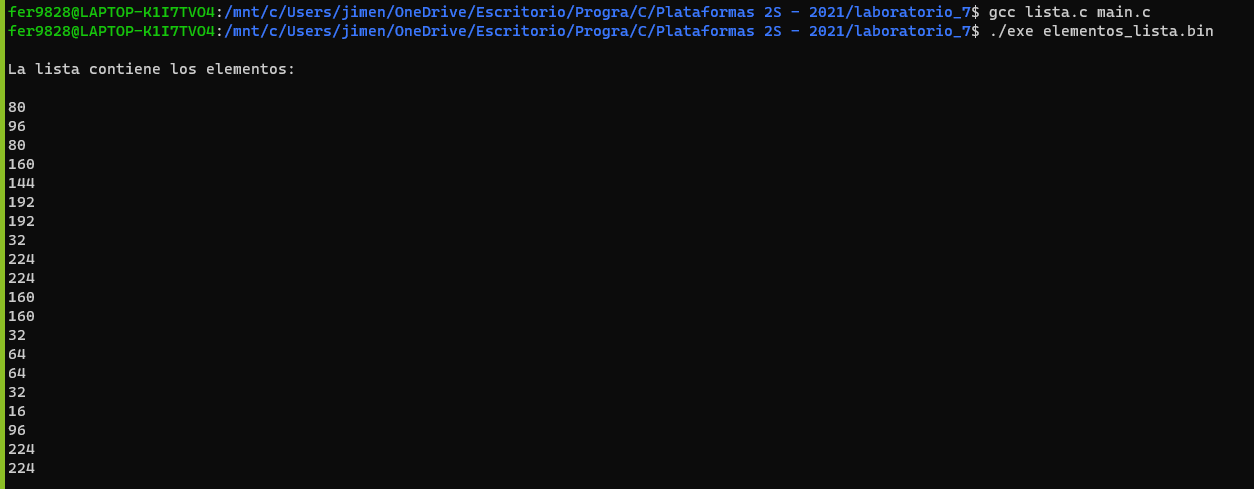
\includegraphics[width=0.9\textwidth]{FotosLabo7/Figura1.png}
    \caption{Funciones printList() y printElement()x. \cite{cap}}
    \label{fig:createList}
\end{figure}



\subsection{Funciones insertElement() y push\_front()}

insertElement(): Esta función agrega un elemento a la lista. Recibe como parámetros el puntero al puntero que a punta al primer elemento de la lista, la posición donde desea insertar el nuevo elemento y el valor entero que desea agregar. Regresa 0 en caso de haber agregado correctamente el elemento, o 1 en caso de no poder localizar la memoria necesaria. Debe reservar memoria.

push\_front(): Esta función regresa un 0 si se logra añadir un calor al principio de la lista, o un 1 si no. Recibe el puntero al primer elemento y el elemento que se desea añadir.

Luego, se procede a probar las distintas funciones implementadas en la lista generada anteriormente. Con la función insertElement() se procede a agregar un elemento a la lista. Además, esta función llama a la función push\_front() ya que se desea que este elemento se agregue en la primera posición de la lista. Es importante mencionar que esta función reserva memoria para este nuevo elemento.

Como se puede apreciar en la Figura 2., se agregó el número entero '786' al inicio de la lista.

\begin{figure}[H]
    \centering
    \center
    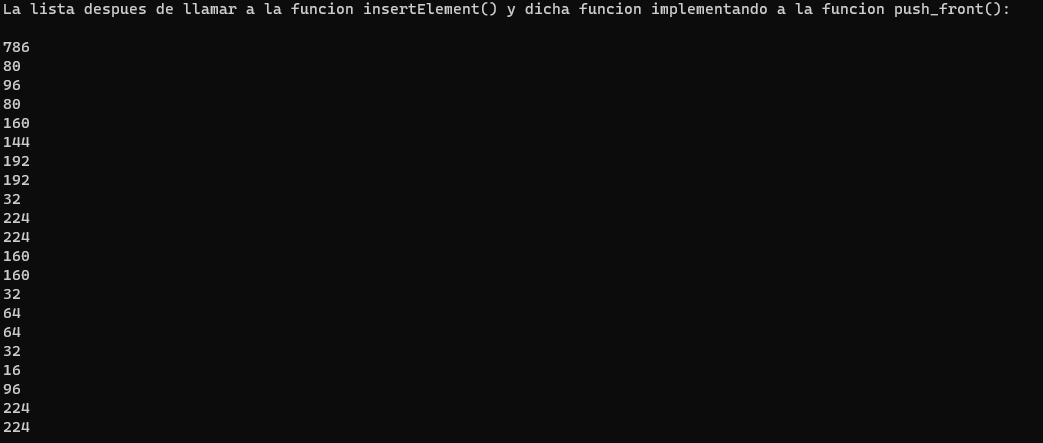
\includegraphics[width=0.9\textwidth]{FotosLabo7/Figura2.png}
    \caption{Funciones insertElement() y push\_front() \cite{cap}}
    \label{fig:writeList}
\end{figure}

\subsection{Funciones pop\_front() y pop\_back()}

pop\_front(): esta función elimina la primera posición de la lista y además regresa el valor entero que estaba almacenado en dicha posici´on. Adem´as debe de hacer los cambios necesarios en la lista para que siga siendo una lista enlazada v´alida. Recibe como par´ametro el puntero al puntero que a punta al primer elemento de la lista. Debe liberar memoria.

pop\_back(): esta función elimina la ´ultima posición de la lista y además regresa el valor entero que estaba almacenado en dicha posición. Además debe de hacer los cambios necesarios en la lista para que siga siendo una lista enlazada válida. Recibe como parámetro el puntero al primer elemento de la lista. Debe liberar memoria.

Se siguen implementando distintas funciones a la lista generada. En este caso se utilizaron las funciones pop\_front() y pop\_back(). El objetivo de estas funciones es eliminar el primer y último elemento de la lista respectivamente además de liberar la memoria.

En la Figura 3. se puede apreciar como el número entero '786' agregado anteriormente y el último número de la lista fueron eliminados.

\begin{figure}[H]
    \centering
    \center
    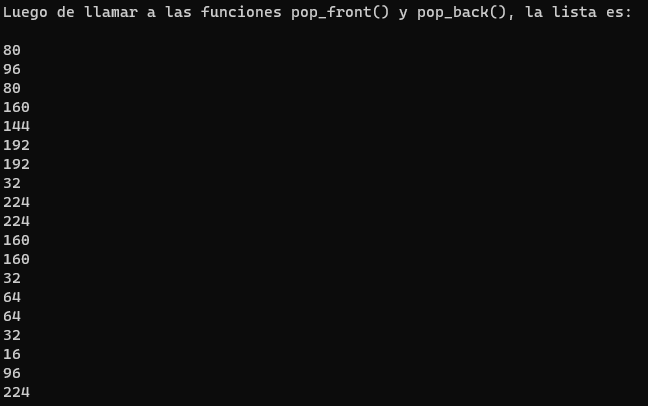
\includegraphics[width=0.9\textwidth]{FotosLabo7/Figura3.png}
    \caption{Funciones pop\_front() y pop\_back() \cite{cap}}
    \label{fig:}
\end{figure}

\subsection{Funciones getElement() y removeElement()}

getElement(): esta función se encarga de regresar el valor de un elemento específico de la lista. Recibe como parámetro el puntero al primer elemento de la lista, la posición que desea obtener y un puntero a int donde se almacenará un 0 en caso de que el valor retornado sea valido o 1 en caso contrario. Un valor no será válido en caso de que el usuario solicite una posición que no existe en la lista.

removeElement(): esta función elimina un elemento de la lista. Recibe como parámetros el puntero al puntero que a punta al primer elemento de la lista y la posición de la lista que desea eliminar. Regresa el valor del elemento eliminado o -1 en caso de haber un error. Debe liberar memoria.

Luego, se procede a llamar las funciones getElement() y removeElement(). En este caso, la función getElement() imprime en la pantalla de la terminal el valor que se encuentra en la posición seleccionada, para este ejemplo se decidió imprimir en pantalla el valor que se encuentra en la posición 15 de la lista. Mientras que la función removeElement() elimina el valor que se encuentra en la posición que se selecciona. Para este caso se decidió eliminar el valor en posición 11, por lo que se eliminó el número entero '160'.



\begin{figure}[H]
    \centering
    \center
    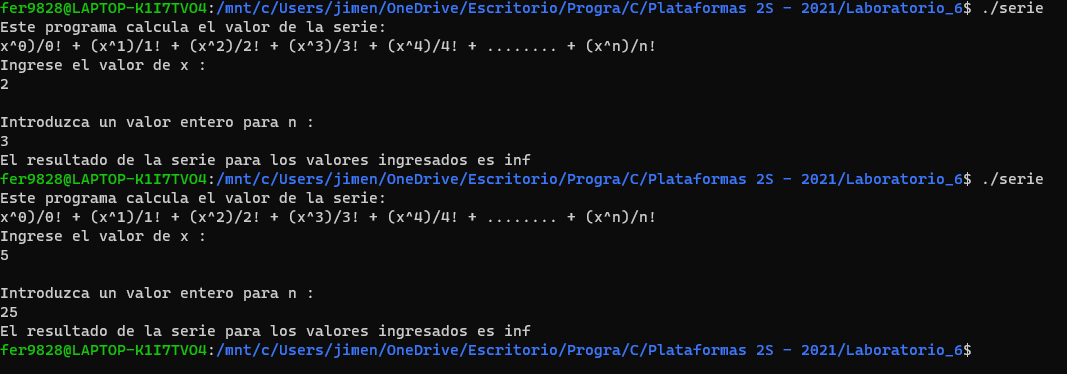
\includegraphics[width=0.9\textwidth]{FotosLabo7/Figura4.png}
    \caption{Funciones getElement() y removeElement() \cite{cap}}
    \label{fig:push_front}
\end{figure}

\subsection{Función writeList()}

Esta función escribe una lista en un archivo de texto plano. Recibe como parámetro el puntero al primer elemento de la lista y la ruta del archivo donde se quiere guardar la lista. Cada elemento de la lista se escribir´a separado por un cambio de l´ınea en el archivo de salida.

Para esta función como bien se describe en el párrafo anterior, para que se ejecute correctamente se debe pasar como argumentos primero el head donde se encuentra la lista y luego un archivo de texto plano para que se pueda guardar la lista.

En la Figura 5. se puede apreciar la correcta ejecución de la función además con el comando \textit{cat} en la terminal se puede imprimir este archivo de texto generado. Y luego en la Figura 6. el archivo de texto plano con la lista guardada.

\begin{figure}[H]
    \centering
    \center
    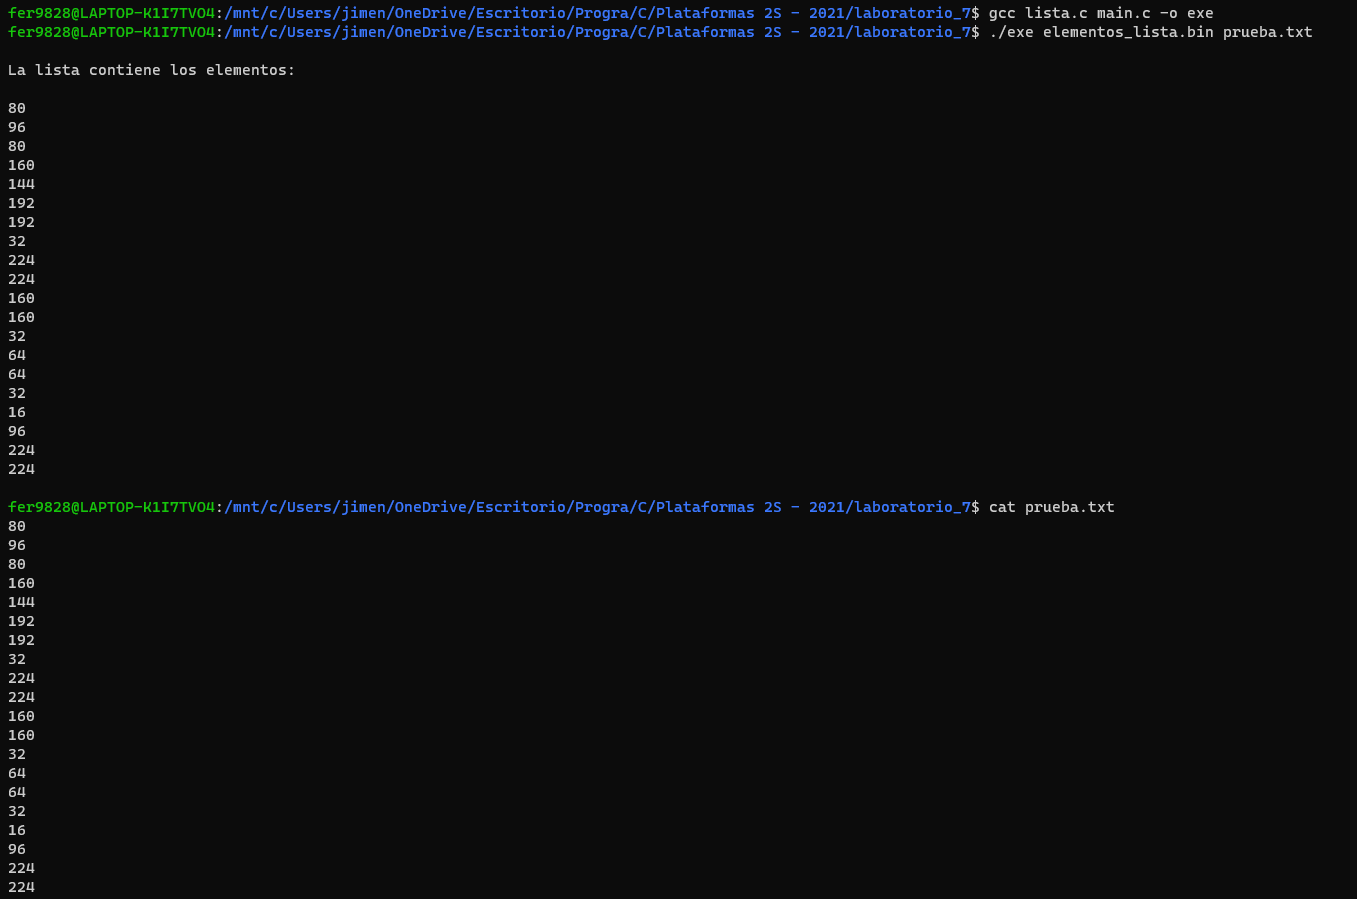
\includegraphics[width=0.9\textwidth]{FotosLabo7/Figura 5.png}
    \caption{Función writeList() \cite{cap}}
    \label{fig:push_front}
\end{figure}

\begin{figure}[H]
    \centering
    \center
    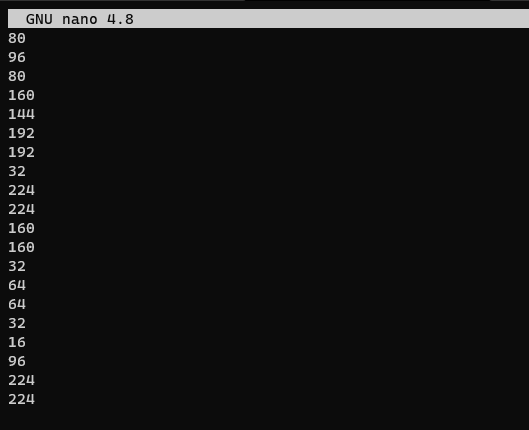
\includegraphics[width=0.9\textwidth]{FotosLabo7/Figura 6.png}
    \caption{Archivo de texto plano \cite{cap}}
    \label{fig:push_front}
\end{figure}

\subsection{Función sort()}

Esta función se encarga de ordenar la lista. Lo realiza de manera ascendente si el \textit{char} recibido como parámetro es ’a’, o de manera descendente en caso de que el \textit{char} recibido sea ’d’. Deja la lista intacta en caso de recibir cualquier otra letra. Además recibe como parámetro el puntero al primer elemento de la lista.

Se puede apreciar en la Figura 8. la función siendo ejecutada sin embargo no se logró obtener el resultado esperado.

\begin{figure}[H]
    \centering
    \center
    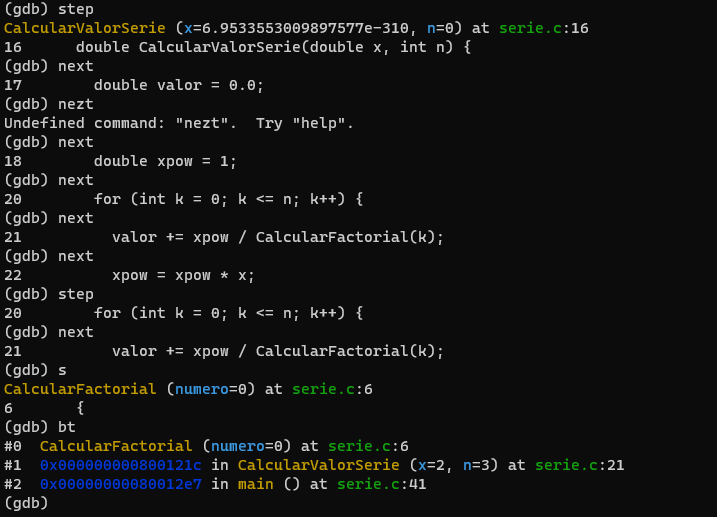
\includegraphics[width=0.9\textwidth]{FotosLabo7/Figura7.png}
    \caption{Función sort() \cite{cap}}
    \label{fig:push_front}
\end{figure}

\subsection{Función freeList()}

Esta función se encarga de liberar toda la memoria que haya sido localizada para la lista. Recibe como único parámetro el puntero al primer elemento dela lista.

En este caso, se puede apreciar en la Figura 8., la ejecución de la función freeList(). En este caso primero se imprimió en pantalla la lista completa con las funciones descritas anteriormente y luego cuando se utiliza la función freeList(), se logra un 0 que demuestra que se logró liberar la memoria correctamente.

\begin{figure}[H]
    \centering
    \center
    \includegraphics[width=0.9\textwidth]{FotosLabo7/FreeList.png}
    \caption{Función freeList() \cite{cap}}
    \label{fig:push_front}
\end{figure}

\vspace{8mm}
\section{Conclusiones y Recomendaciones}

En el presente Laboratorio se logró demostrar la utilidad e importancia de las listas enlazadas y \textit{structs}. El manejo de dichas herramientas se vuelven esencial para poder trabajar y manejar datos. Esto debido a que se puede trabajar con memoria dinámica y asignarle tamaños específicos a las variables. Además se logró observar que con el uso de \textit{structs} se puede manipular datos de diferentes tipos dentro de una misma lista de datos, algo que no era posible con el uso de de arreglos.

Con el desarrollo de este último laboratorio se logró complementar y concluir todo lo aprendido en el curso sobre el lenguaje de programación C. Se logró aprender las bases sobre las funcionalidades y aplicaciones que se pueden lograr con la ayuda de la programación además de poder desarrollar un entendimiento más analítico de una amplia variedad de temas en informática.  



\begin{thebibliography}{}
\bibitem{cap}
Creación propia.

\bibitem{pres}
Villalta, M.(2021) \textit{C: compiladores, IDE, herramientas}.  

\bibitem{meza}
Meza, J. (2021). Estructuras de datos en C++: Vectores, matrices y punteros. Programarya.com. Retrieved 22 November 2021, from https://www.programarya.com/Cursos/C++/Estructuras-de-Datos.

\bibitem{ccm}
CCM Benschmark Group. (17 de noviembre de 2021) \textit{GDB Command Reference}. https://es.ccm.net/faq/2842-la-lista-enlazada-simple


\end{thebibliography}

%Formato para añadir imagenes

\end{document}